\documentclass{report}
\usepackage[T1]{fontenc} % Fontes T1
\usepackage[utf8]{inputenc} % Input UTF8
\usepackage[backend=biber, style=ieee]{biblatex} % para usar bibliografia
\usepackage{csquotes}
\usepackage[portuguese]{babel} %Usar língua portuguesa
\usepackage{blindtext} % Gerar texto automaticamente
\usepackage[printonlyused]{acronym}
\usepackage{hyperref} % para autoref
\usepackage{graphicx}


\bibliography{bibliografia}


\begin{document}
%%
% Definições
%
\def\titulo{Projeto Final de LSD }
\def\data{17 de junho de 2021}
\def\autores{Guilherme Craveiro, Rafael Pinto}
\def\autorescontactos{(103574) gjscraveiro@ua.pt, (103379) rafaelpbpinto@ua.pt}
\def\versao{Versão 1}
\def\departamento{Departamento de Eletrónica, Telecomunicações e Informática}
\def\empresa{Universidade de Aveiro}
\def\logotipo{ua.pdf}
%
%%%%%% CAPA %%%%%%
%
\renewcommand{\contentsname}{Índice}
\begin{titlepage}

\begin{center}
%
\vspace*{50mm}
%
{\Huge \titulo}\\ 
%
\vspace{10mm}
%
{\Large \empresa}\\
%
\vspace{10mm}
%
{\LARGE \autores}\\ 
%
\vspace{30mm}
%
\begin{figure}[h]
\center
\includegraphics{\logotipo}
\end{figure}
%
\vspace{30mm}
\end{center}
%
\begin{flushright}
\versao
\end{flushright}
\end{titlepage}

%%  Página de Título %%
\title{%
{\Huge\textbf{\titulo}}\\
{\Large \departamento\\ \empresa}
}
%
\author{%
    \autores \\
    \autorescontactos
}
%
\date{\data}
%
\maketitle

\pagenumbering{roman}

\tableofcontents
% \listoftables     % descomentar se necessário
% \listoffigures    % descomentar se necessário


%%%%%%%%%%%%%%%%%%%%%%%%%%%%%%%
\clearpage
\pagenumbering{arabic}

%%%%%%%%%%%%%%%%%%%%%%%%%%%%%%%%
\chapter{Introdução}
\label{chap.introducao}

\ac{vhdl} é uma linguagem usada para modelar o comportamento e a estrutura de sistemas digitais em, por exemplo, \ac{fpga}. De forma muito resumida, \ac{fpga} é uma matriz de blocos lógicos interligados de modo inteligente que podem ser reprogramados para a aplicação desejada.

Este relatório tem como objetivo explicar o funcionamento da máquina automática de oferta de produtos desenvolvida no nosso projeto. Para que a máquina funcionasse foi necessário a implementação de código em \ac{vhdl} e procedeu-se a vários testes na \ac{fpga} e à análise dos mesmos.

A máquina disponibiliza 3 bebidas diferentes das quais podemos selecionar uma através de \textit{switches}. Após a disponibilização da bebida o utilizador pode ainda entrar no modo "Modo Escolha tamanho das garrafas", onde pode escolher o tamanho da garrafa, 25cl, 33cl, 50cl ou 10dl. Por defeito está configurado para 33cl. A máquina tem ainda um RESET global que coloca a máquina no estado inicial.
 
\chapter{Arquitetura}
\label{chap.arquitetura}
descrição da estrutura conceptual do sistema com pelo menos uma figura ilustrativa

\begin{figure}[h]
    \centering
    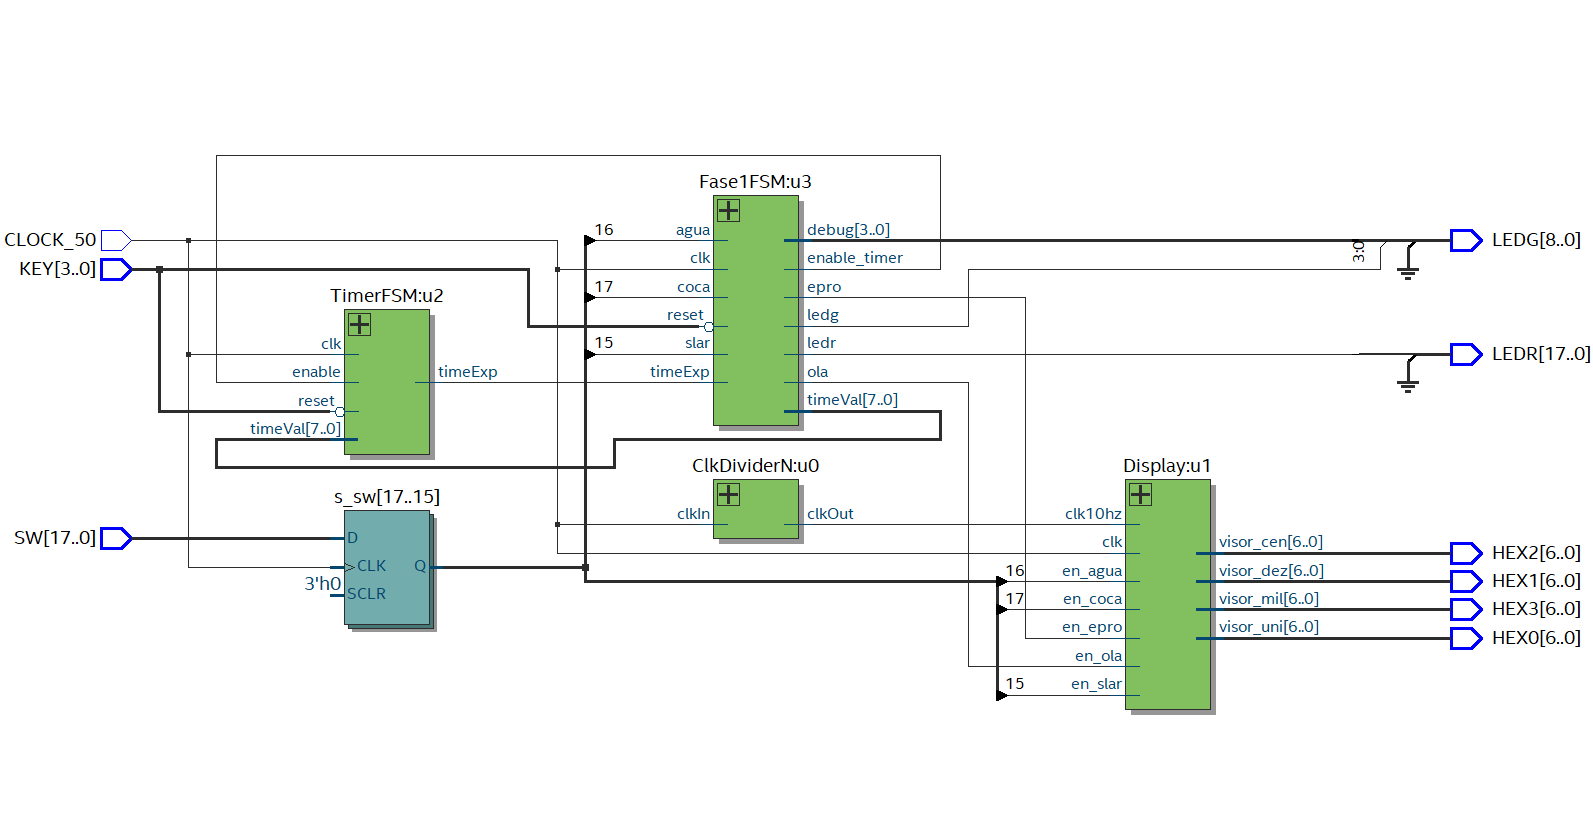
\includegraphics[width=10cm]{Fase1Estrutura.png}
    \caption{Estrutura da Fase 1}
    \label{fig:Fase1Estrutura}
\end{figure}


\chapter{Implementação}
\label{chap.implementação}
incluindo representação gráfica das máquinas de estado finitos
implementadas – se aplicável, aspetos de implementação mais relevantes e ligação a
periféricos do kit

\chapter{Validação}
\label{chap.validação}
simulação dos principais módulos

\chapter{Manual do utilizador}


\chapter{Conclusões}
\label{chap.conclusao}
Apresenta conclusões.

\chapter*{Contribuições dos autores}
Resumir aqui o que cada autor fez no trabalho.
Usar abreviaturas para identificar os autores,
por exemplo AS para António Silva.
No fim indicar a percentagem de contribuição de cada autor.

%%%%%%%%%%%%%%%%%%%%%%%%%%%%%%%%%
\chapter*{Acrónimos}
\begin{acronym}
\acro{ua}[UA]{Universidade de Aveiro}
\acro{miect}[MIECT]{Mestrado Integrado em Engenharia de Computadores e Telemática}
\acro{lei}[LEI]{Licenciatura em Engenharia Informática}
\acro{glisc}[GLISC]{Grey Literature International Steering Committee}
\acro{lsd}[LSD]{Laboratórios de Sistemas Digitais}
\acro{vhdl}[VHDL]{VHSIC Hardware Description Language}
\acro{fpga}[FPGA]{Field Programmable Gate Array}
\end{acronym}


%%%%%%%%%%%%%%%%%%%%%%%%%%%%%%%%%
\printbibliography

\end{document}